% MATH 201 Lab notes (c) by Carlos Contreras And Philippe Gaudreau
% MATH 201 Lab notes is licensed under a 
% Creative Commons Attribution 4.0 International license.
% CC BY 4.0

% You should have received a copy of the license along with this
% work. If not, see <http://creativecommons.org/licenses/by/4.0/>.

\documentclass[11pt]{article}
% MATH 201 Lab notes (c) by Carlos Contreras And Philippe Gaudreau
% MATH 201 Lab notes is licensed under a 
% Creative Commons Attribution 4.0 International license.
% CC BY 4.0

% You should have received a copy of the license along with this
% work. If not, see <http://creativecommons.org/licenses/by/4.0/>.

%% libraries
\usepackage[utf8x]{inputenc}
\usepackage{xcolor}
\usepackage[left=1.5cm,right=1.5cm,top=2.0cm,bottom=1.5cm,headheight=110pt]{geometry}
\usepackage{amsmath}
\usepackage{amssymb}
\usepackage{graphicx}
\usepackage{xifthen}
\usepackage{sverb}
\usepackage{fancyhdr}
\usepackage{mdframed}
\usepackage{textcomp}

%%%%%%%%%%%%%%%%%%%%%%%%%%%%%%%%%%%%%%%%%%%%%%%%%%%%%%%%%%%%%%%%%%%%%%%
% PDF compiling
\usepackage{ifpdf}
\ifpdf %
        \DeclareGraphicsExtensions{.pdf}%
\else %
        \DeclareGraphicsExtensions{.eps,.ps}%
\fi

%%%%%%%%%%%%%%%%%%%%%%%%%%%%%%%%%%%%%%%%%%%%%%%%%%%%%%%%%%%%%%%%%%%%%%%
% Figures path
\graphicspath{{figures/}}

%%%%%%%%%%%%%%%%%%%%%%%%%%%%%%%%%%%%%%%%%%%%%%%%%%%%%%%%%%%%%%%%%%%%%%%
% Problem counter
\newcounter{Problem}
\setcounter{Problem}{0}

%%%%%%%%%%%%%%%%%%%%%%%%%%%%%%%%%%%%%%%%%%%%%%%%%%%%%%%%%%%%%%%%%%%%%%%
% Definitions
\def\LabSolutions{\clearpage \newpage \begin{center} {\Large \it Solutions} \end{center} \setcounter{Problem}{0}}
\def\QuizSolutions{\newpage \begin{center} {\Large \it Solutions} \end{center} \setcounter{Problem}{0}}
\def\degree{\textdegree}
\def\grade#1{\begin{flushright} {\small [#1]}\\ \end{flushright} \vspace{-10pt}}
\def\codecolor{red!50!black}
\def\code#1{\textcolor{\codecolor}{\tt #1}}
\def\examname#1{%
                \ifnum\value{page}>1%
                    \newpage%
                \else%
                    \vspace*{5pt}%
                \fi%
                \large \textbf{#1} \setcounter{Problem}{0}\vspace{10pt}}
\def\topic#1{\par\needspace{2\baselineskip} \noindent \textsl{\footnotesize #1}}

 
%%%%%%%%%%%%%%%%%%%%%%%%%%%%%%%%%%%%%%%%%%%%%%%%%%%%%%%%%%%%%%%%%%%%%%%
% Environments
\newenvironment{problem}%
     {\stepcounter{Problem}%
      \begin{list}{\textbf{\arabic{Problem}}.~}{}%
      \item}%
     {\end{list}\vspace*{5pt}}

\newenvironment{solution}%
     {\indent \textit{Solution} \newline}%
     {\begin{flushright}$\blacksquare$\end{flushright}}

\newenvironment{preamble}%
     {\vspace*{1em}\begin{mdframed}[leftmargin=1cm,rightmargin=1cm]}%
     {\end{mdframed}\vspace*{1em}}

\newenvironment{multchoice}%
     {\begin{enumerate} \addtolength{\leftskip}{2em} \renewcommand{\labelenumi}{(\alph{enumi})}}
     {\end{enumerate}}

\newenvironment{formulaitem}%
     {\setlength{\leftmargini}{1.5em}\begin{itemize}%
      \setlength\itemindent{-\itemindent}%
      \renewcommand{\labelitemi}{$\rightarrow$}}%
     {\end{itemize}}


%%%%%%%%%%%%%%%%%%%%%%%%%%%%%%%%%%%%%%%%%%%%%%%%%%%%%%%%%%%%%%%%%%%%%%%
% New theorems
\newtheorem{theorem}{Theorem}


\makeatletter

%%%%%%%%%%%%%%%%%%%%%%%%%%%%%%%%%%%%%%%%%%%%%%%%%%%%%%%%%%%%%%%%%%%%%%%
%% New commands
\newcommand*{\course}[1]{\gdef\@course{#1}}
\newcommand*{\coursecode}[1]{\gdef\@coursecode{#1}}
\newcommand*{\term}[1]{\gdef\@term{#1}}
\newcommand*{\instructor}[1]{\gdef\@instructor{#1}}
\newcommand*{\lqnumber}[1]{\gdef\@lqnumber{#1}}
\newcommand*{\labtitle}[1]{\gdef\@labtitle{#1}}
\newcommand*{\quizversion}[1]{\gdef\@quizversion{#1}}
\newcommand*{\probleminfo}[1]{\noindent \textsl{\footnotesize #1}}

% Title header for labs
\newcommand\makelabtitle{%
  \begin{flushleft}%
  {\scshape \@coursecode~\@course~-- University of Alberta}\\%
  {\scshape \@term~-- Labs -- \@instructor}\\%
  {\scshape Authors: Carlos Contreras and Philippe Gaudreau}%
  \end{flushleft}%
  \begin{center}%
  {\Large \bf \@lqnumber:~\@labtitle}%
  \end{center}%
  \thispagestyle{empty}%
  \global\let\@course\@empty%
  \global\let\@labtitle\@empty%
}

% Title header for quizzes
\newcommand\makequiztitle{%
  \begin{flushleft}%
  {\scshape \@coursecode~\@course~-- University of Alberta}\\%
  {\scshape \@term~-- Labs -- \@instructor}\\%
  \end{flushleft}%
  \begin{center}%
  {\Large \bf \@lqnumber} \marginpar{\tiny\tt [\@quizversion]}%
  \end{center}%
  \thispagestyle{empty}%
  \global\let\@course\@empty%
  \global\let\@quizversion\@empty%
}

%%%%%%%%%%%%%%%%%%%%%%%%%%%%%%%%%%%%%%%%%%%%%%%%%%%%%%%%%%%%%%%%%%%%%%%
% Fancy header package
\fancyhead[L]{\small {\scshape \@coursecode~-- \@lqnumber~-- \@term~-- \@instructor}}
\pagestyle{fancy}

\makeatother


\usepackage{hyperref}
\usepackage{cancel}

\usepackage{pgfplots}

\begin{document}

\course{Differential Equations}
\coursecode{MATH 201}
\term{Winter 2018}
\instructor{Carlos Contreras}
\lqnumber{Lab 11}
\labtitle{Fourier series}
\makelabtitle



\topic{Fourier series ($[-L,L]$)}
\begin{problem}
Compute the Fourier series for the given function on the specific interval
\begin{eqnarray*}
f(x) = x^2 , \quad -3<x<3.
\end{eqnarray*}
\end{problem}


\begin{problem}
Compute the Fourier series for the given function on the specific interval
\begin{eqnarray*}
f(x) = x , \quad -\pi<x<\pi,
\end{eqnarray*}
and sketch a graph of the Fourier series on the domain $-3\pi<x<3\pi$.
\end{problem}

\begin{problem}
Find the Fourier series of the piecewise function $f$ defined as
\begin{equation*}
f(x) = \left\{ \begin{array}{lr} 0, & -1 \leq x < 0 \\ x^{2}, & 0 \leq x < 1 \end{array} \right.,
\end{equation*}
sketch a graph, and determine its sum for all $|x|\leq 1$.
\end{problem}

\topic{Fourier sine and cosine series ($[0, L]$)}
\begin{problem}
Compute the Fourier sine series and Fourier cosine series for the given function
\begin{equation*}
f(x) = x-x^2, \quad 0<x<1
\end{equation*}
\end{problem}


%%%%%%%%%%%%%%%%%%%%%%%%%%%%%%%%%%%%%%%%%%%%%%%%%%%%%%%%%%%%%%%%%%%%%%%%%%%%%%%%%%%%%%%%%%%%%%%%%%%



\LabSolutions


Theory and problems from: Nagel, Saff \& Sneider, \textit{Fundamentals of Differential Equations}, Eighth Edition, Adisson--Wesley.

\begin{preamble}
\begin{formulaitem}

\item The \textbf{Fourier series} of $f(x)$ on the interval $[-L, L]$ is 
\[F(x) = \dfrac{a_{0}}{2} + \sum_{n=1}^{\infty} \left[ a_{n}\cos\left(\dfrac{n\pi x}{L}\right)+b_{n}\sin\left(\dfrac{n\pi x}{L}\right) \right],\]
where
\[a_{n} = \dfrac{1}{L} \int_{-L}^{L} f(x)\cos\left(\dfrac{n\pi x}{L}\right) dx, \qquad n\geq 0, \]
and 
\[b_{n} = \dfrac{1}{L} \int_{-L}^{L} f(x)\sin\left(\dfrac{n\pi x}{L}\right) dx, \qquad n\geq 1.\]

Moreover, the sum converges  for all $|x|\leq L$ to

\begin{equation*}
F(x) = \begin{cases} f(x) & \text{if $-L<x<L$ and $f$ is continuous at $x$,} \\[0.5em]
                                 \dfrac{f(x-)+f(x+)}{2} & \text{if $-L<x<L$ and $f$ is discontinuous at $x$,} \\[0.5em]
                                 \dfrac{f(-L+)+f(L-)}{2} & \text{if $x=L$ or $x=-L$.} \end{cases} 
\end{equation*}

\item Properties of \textbf{even} ($f(-x)=f(x)$) and \textbf{odd} ($-f(-x)=f(x)$) \textbf{functions}
\begin{enumerate}
     \item even $\pm$ even = even, \quad even $\times$ even = even
     \item odd $\pm$ odd = odd, \quad odd $\times$ odd = even
     \item odd $\pm$ even = none, \quad odd $\times$ even = odd
     \item for $f(x)$ even $\int_{-L}^{L}f(x)dx= 2\int_{0}^{L}f(x)dx$
     \item for $f(x)$ odd $\int_{-L}^{L}f(x)dx= 0$
     \item for $f(x)$ even $b_{n}=0$, and $a_{n}=2\int_{0}^{L}f(x)\cos\left( \tfrac{n\pi x}{L} \right)dx$.
     \item for $f(x)$ odd  $a_{n}=0$, and $b_{n}=2\int_{0}^{L}f(x)\sin\left( \tfrac{n\pi x}{L} \right)dx$.
\end{enumerate}

\item The \textbf{Fourier Sine Series} of $f(x)$ on $[0,L]$ is

\begin{equation*}
S(x) = \sum_{n=1}^{\infty} b_{n} \sin \left(\dfrac{n\pi x}{L}\right)
\end{equation*}

where 

\begin{equation*}
b_{n} = \dfrac{2}{L} \int_{0}^{L} f(x) \sin \left( \dfrac{n \pi x}{L} \right) dx, \quad n\geq 1.
\end{equation*}

\item The \textbf{Fourier Cosine series} of $f(x)$ on $[0, L]$
\begin{equation*}
C(x) = \frac{a_{0}}{2}+\sum_{n=1}^{\infty} a_{n} \cos \left(\dfrac{n\pi x}{L}\right)
\end{equation*}
where
\begin{equation*}
a_{n}=\frac{2}{L}\int_{0}^{L}f(x)\cos \left(\dfrac{n\pi x}{L}\right) dx, \quad n\geq 0.
\end{equation*}
\end{formulaitem}
\end{preamble}








\begin{problem}
Compute the Fourier series for the given function on the specific interval
\begin{eqnarray*}
f(x) = x^2 , \quad -3<x<3.
\end{eqnarray*}
\end{problem}
\begin{solution}
We want to write $f(x)$ in the form
\begin{eqnarray*}
F(x) = \dfrac{a_{0}}{2} + \sum_{n=1}^{\infty} \left[ a_{n}\cos\left(\dfrac{n\pi x}{3}\right)+b_{n}\sin\left(\dfrac{n\pi x}{3}\right) \right]
\end{eqnarray*}
Since $f(x)$ is an even function, we know that
\begin{eqnarray*}
b_{n} = \dfrac{1}{3} \int_{-3}^{3} x^2\sin\left(\dfrac{n\pi x}{3}\right) dx =0, \quad {\rm for} \quad n =1,2,3,\ldots
\end{eqnarray*}
Hence, all we need to do is find the coefficients $a_{n}$ Since $f(x)$ is an even function, we have for $n =0,1,2,3,\ldots$ :
\begin{equation*}
a_{n} = \dfrac{1}{3} \int_{-3}^{3} x^2\cos\left(\dfrac{n\pi x}{3}\right) dx = \dfrac{2}{3} \int_{0}^{3} x^2\cos\left(\dfrac{n\pi x}{3}\right) dx \\
\end{equation*}
First, we find $a_{0}$
\begin{eqnarray*}
a_{0} & = & \dfrac{2}{3}  \int_{0}^{3} x^2 dx \\
& = & \dfrac{2}{3}  \left[\dfrac{x^3}{3}\right]_{0}^{3} \\
& = &\dfrac{2}{3} \left( \dfrac{3^3}{3} \right)\\
& = & 6
\end{eqnarray*}
Now, to find $a_{n}$. We use integration by parts twice to solve this integral
\begin{eqnarray*}
a_{n} & = & \dfrac{2}{3}\int_{0}^{3} x^2\cos\left(\dfrac{n\pi x}{3}\right) dx \\
& = &  \dfrac{2}{3}\left[(x^2)\left(\dfrac{3}{n\pi} \sin\left(\dfrac{n\pi x}{3}\right)\right) \right]_{0}^{3} - \dfrac{2}{3} \int_{0}^{3} (2x)\left(\dfrac{3}{n\pi} \sin\left(\dfrac{n\pi x}{3}\right)\right) dx \\
& = &  0 - \dfrac{4}{n\pi} \int_{0}^{3} x \sin\left(\dfrac{n\pi x}{3}\right) dx \\
& = &   -\dfrac{4}{n\pi} \left[ (x) \left(-\dfrac{3}{n\pi} \cos\left(\dfrac{n\pi x}{3}\right)\right) \right]_{0}^{3} + \dfrac{4}{n\pi} \int_{0}^{3} (1) \left(-\dfrac{3}{n\pi} \cos\left(\dfrac{n\pi x}{3}\right)\right) dx \\
& = &   -\dfrac{4}{n\pi} \left[ -\dfrac{9}{n\pi} \cos\left(n\pi\right) - 0 \right] - \dfrac{12}{n^2\pi^2} \int_{0}^{3}  \cos\left(\dfrac{n\pi x}{3}\right) dx \\
& = &   \dfrac{36}{n^2\pi^2} \cos\left(n\pi\right) + \dfrac{12}{n^2\pi^2} \left[  \dfrac{3}{n\pi} \sin\left(\dfrac{n\pi x}{3}\right) \right]_{0}^{3} \\
& = &   \dfrac{36}{n^2\pi^2} \cos\left(n\pi\right) + 0 \\
& = &   \dfrac{36}{n^2\pi^2} (-1)^n \\
& = &   \dfrac{36(-1)^{n}}{n^2\pi^2}  \\
\end{eqnarray*}
Hence, after all this laborious work, we obtain our solution
\begin{eqnarray*}
\boxed{F(x) =  x^2 = 3 + \sum_{n=1}^{\infty}  \dfrac{36(-1)^{n}}{n^2\pi^2} \cos\left(\dfrac{n\pi x}{3}\right)}.
\end{eqnarray*}
\end{solution}


\begin{problem}
Compute the Fourier series for the given function on the specific interval
\begin{eqnarray*}
f(x) = x , \quad -\pi<x<\pi,
\end{eqnarray*}
and sketch a graph of the Fourier series on the domain $-3\pi<x<3\pi$.
\end{problem}
\begin{solution}
First, note that $f(x)$ is \textsl{odd}, and $L=\pi$.
We want to write $f(x)$ in the form
\begin{eqnarray*}
F(x) = \dfrac{a_{0}}{2} + \sum_{n=1}^{\infty} \left[ a_{n}\cos\left(n x\right)+b_{n}\sin\left(n x\right) \right]
\end{eqnarray*}
Since $f(x)$ is an odd function, we know that
\begin{eqnarray*}
a_{n} = \dfrac{1}{\pi} \int_{-\pi}^{\pi} x\cos\left(n x\right) dx =0, \quad {\rm for} \quad n =1,2,3,\ldots,
\end{eqnarray*}
and
\begin{eqnarray*}
a_{0} = \dfrac{1}{\pi} \int_{-\pi}^{\pi} x dx =0.
\end{eqnarray*}
For $b_{n}$ we use one integration by parts.
\begin{align*}
b_{n}& = \frac{1}{\pi}\int_{-\pi}^{\pi} x\sin\left(n x\right) dx = \frac{2}{\pi}\int_{0}^{\pi} x\sin\left(n x\right) dx \\
     & = \frac{2}{\pi}\left[ -\frac{x}{n}\cos (nx) |^{\pi}_{0} + \frac{1}{n}\int_{0}^{\pi} \cos\left(n x\right) dx\right] \\
     & = \frac{2}{\pi}\left[ -\frac{\pi}{n}\cos (n\pi)  + \frac{1}{n^{2}}\sin (nx)|^{\pi}_{0} \right] = \frac{(-1)^{n+1}2}{n}.
\end{align*}
Thus,
\[\boxed{F(x) = \sum_{n=1}^{\infty}\frac{(-1)^{n+1}2}{n}\sin(nx)}.\]
To sketch a graph we extend periodically $f(x)$ and redefined points of discontinuity to the midpoint.
\begin{figure}[h]
\begin{center}
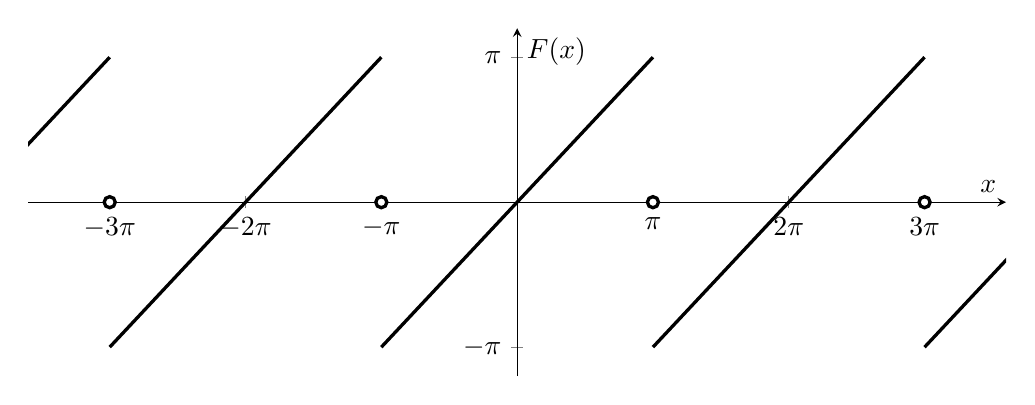
\begin{tikzpicture}
     \begin{axis}[width=14cm, height=6cm,
                  xlabel={$x$}, ylabel={$F(x)$},
                  xmin=-3, xmax=3,ymin=-1, ymax=1, 
                  ytick={-1,0,1}, xtick={-3,-2,-1,0,1,2,3},
                  yticklabels={$-\pi$, $0$, $\pi$}, xticklabels={$-3\pi$, $-2\pi$, $-\pi$, $0$, $\pi$, $2\pi$, $3\pi$},
                  axis lines = middle, enlargelimits = true,
                  every axis plot/.append style={very thick}]
               \addplot[domain=-4:-3] {x+4};
               \addplot[mark=*, fill=white] coordinates {(-3,.0)};
               \addplot[domain=-3:-1] {x+2};
               \addplot[mark=*, fill=white] coordinates {(-1,.0)};
               \addplot[domain=-1:1] {x};
               \addplot[mark=*, fill=white] coordinates {(1,.0)};
               \addplot[domain=1:3] {x-2};
               \addplot[mark=*, fill=white] coordinates {(3,.0)};
               \addplot[domain=3:4] {x-4};
     \end{axis}
\end{tikzpicture}
\end{center}
\caption{Sketch of Fourier series of $f(x)$ for $-3\pi<x<3\pi$.}
\label{fig:prob2}
\end{figure}

\end{solution}



\begin{problem}
Find the Fourier series of the piecewise function $f$ defined as
\begin{equation*}
f(x) = \left\{ \begin{array}{lr} 0, & -1 \leq x < 0 \\ x^{2}, & 0 \leq x < 1 \end{array} \right.,
\end{equation*}
sketch a graph, and determine its sum for all $|x|\leq 1$.
\end{problem}
\begin{solution}
Note that $f(x)$ is not even nor odd. Hence, we have to compute each term in the Fourier expansion
\[F(x) = \frac{a_{0}}{2}+\sum_{n=1}^{\infty}a_{n}\cos\left(n\pi x\right) + b_{n}\sin \left(n\pi x\right),\]
where
\begin{equation*}
\begin{split}
a_{0} & = \int_{-1}^{1}f(x)dx = \int_{0}^{1}x^{2}dx = \frac{1}{3}
\end{split}
\end{equation*}


\begin{equation*}
\begin{split}
a_{n} & = \int_{-1}^{1}f(x)\cos \left(n\pi x\right) dx = \int_{0}^{1}x^{2}\cos \left(n\pi x\right) dx \\
      & = \cancelto{0}{\left.\frac{x^{2}\sin \left(n\pi x\right)}{n\pi}\right|_{0}^{1}} - \int_{0}^{1}\frac{2x\sin \left(n\pi x\right)}{n\pi}dx \\
      & = \left. \frac{2x\cos \left(n\pi x\right)}{n^{2}\pi^{2}}\right|_{0}^{1} - \int_{0}^{1} \frac{2\cos \left(n\pi x\right)}{n^{2}\pi^{2}}dx \\
      & = \frac{2(-1)^{n}}{n^{2}\pi^{2}} + \cancelto{0}{\left. \frac{2\sin \left(n\pi x\right)}{n^{3}\pi^{3}}\right|_{0}^{1}} = \frac{2(-1)^{n}}{n^{2}\pi^{2}}
\end{split}
\end{equation*}


\begin{equation*}
\begin{split}
b_{n} & = \int_{-1}^{1}f(x)\sin \left(n\pi x\right)dx = \int_{0}^{1}x^{2}\sin \left(n\pi x\right)dx \\
      & = -\left.\frac{x^{2}\cos \left(n\pi x\right)}{n\pi}\right|_{0}^{1} + \int_{0}^{1}\frac{2x\cos \left(n\pi x\right)}{n\pi} dx \\
      & = -\frac{(-1)^{n}}{n\pi} + \left.\frac{2x\sin\left(n\pi x\right)}{n^{\pi^{2}}}\right|_{0}^{1} - \int_{0}^{1}\frac{2x\sin\left(n\pi x\right)}{n^{2}\pi^{2}}dx \\
      & = -\frac{(-1)^{n}}{n\pi} + \left.\frac{2\cos\left(n\pi x\right)}{n^{3}{\pi^{3}}}\right|_{0}^{1} \\
      & = -\frac{(-1)^{n}}{n\pi} + \frac{2((-1)^{n}-1)}{n^{3}\pi^{3}}
\end{split}
\end{equation*}

Thus, the Fourier series of $f(x)$ is
\[\boxed{F(x) = \frac{1}{6}+\sum_{n=1}^{\infty}\left[\left( \frac{2(-1)^{n}}{n^{2}\pi^{2}} \right)\cos\left(n\pi x\right) + \left( -\frac{(-1)^{n}}{n\pi} + \frac{2((-1)^{n}-1)}{n^{3}\pi^{3}} \right)\sin \left(n\pi x\right)\right]}.\]

A sketch of the graph is shown in Figure \ref{fig:prob3}. 
\begin{figure}[h]
\begin{center}
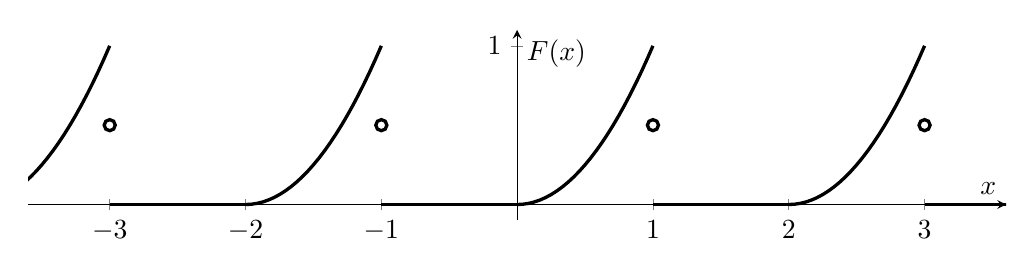
\begin{tikzpicture}
     \begin{axis}[width=14cm, height=4cm,
                  xlabel={$x$}, ylabel={$F(x)$},
                  xmin=-3, xmax=3,ymin=0, ymax=1, 
                  ytick={-1,0,1}, xtick={-3,-2,-1,0,1,2,3},
                  axis lines = middle, enlargelimits = true,
                  every axis plot/.append style={very thick}]
               \addplot[domain=-4:-3] {(x+4)^2};
               \addplot[mark=*, fill=white] coordinates {(-3,.5)};
               \addplot[domain=-3:-2] {0};
               \addplot[domain=-2:-1] {(x+2)^2};
               \addplot[mark=*, fill=white] coordinates {(-1,.5)};
               \addplot[domain=-1:0] {0};
               \addplot[domain=0:1] {x^2};
               \addplot[mark=*, fill=white] coordinates {(1,.5)};
               \addplot[domain=1:2] {0};
               \addplot[domain=2:3] {(x-2)^2};
               \addplot[mark=*, fill=white] coordinates {(3,.5)};
               \addplot[domain=3:4] {0};
     \end{axis}
\end{tikzpicture}
\end{center}
\caption{Sketch of Fourier series of $f(x)$ including 3 periods.}
\label{fig:prob3}
\end{figure}


To find its sum on $[-1,1]$, we find what happens on the points of discontinuity\footnote{If $f(x)$ is discontinuous at $x=a$, $f(a+)$ and $f(a-)$ are the values of the function to the right and left of $a$, respectively.} of $f(x)$, i.e., $x=-1$, and $x=1$ (knowing the graph of $F(x)$ in Figure \ref{fig:prob3} definitely helps here). 

At $x=-1$,
\[F(-1)=\dfrac{f(-1+)+f(1-)}{2}=\frac{0+1^2}{2}=\dfrac{1}{2},\]
which is the same value at $x=1$,
\[F(1)=\dfrac{f(-1+)+f(1-)}{2}=\dfrac{1}{2}.\]
At $x=0$, there is no need to find the value of the sum because the $f(x)$ is continuous at this point.

Hence, the sum for all $|x|\leq1$ is 
\begin{equation*}
\boxed{F(x) = \left\{ \begin{array}{lr} \frac{1}{2}, & x=-1 \\
                                 0, & -1 < x < 0 \\
                                 x^{2}, & 0 \leq x < 1 \\
                                 \frac{1}{2}, & x=1 \end{array} \right..}
\end{equation*}


\end{solution}





\begin{problem}
Compute the Fourier sine series for the given function
\begin{equation*}
f(x) = x-x^2, \quad 0<x<1
\end{equation*}
\end{problem}

\begin{solution}
\textbf{Note:} the given domain is of the form $[0, L]$ instead of $[-L, L]$. In which case the problem is either to find the Fourier Sine series (also called odd extension of $f(x)$ to $[-L, L]$) or the Fourier Cosine series (also called even extension of $f(x)$ to $[-L, L]$).

The Fourier Sine Series of $f(x)$ on $[0,L]$ is

\begin{equation*}
S(x) = \sum_{n=1}^{\infty} b_{n} \sin \left(\dfrac{n\pi x}{L}\right)
\end{equation*}

where 

\begin{equation*}
b_{n} = \dfrac{2}{L} \int_{0}^{L} f(x) \sin \left( \dfrac{n \pi x}{L} \right) {\rm d} x, \quad n=1,2,3,\ldots
\end{equation*}

In our case, we have $L=1$. Let's calculate $b_{n}$.

\begin{eqnarray*}
b_{n} & = & 2 \int_{0}^{1} (x-x^2) \sin \left( n \pi x\right) {\rm d} x \\
 & = & 2 \left[(x-x^2)\left(- \dfrac{\cos(n \pi x)}{n \pi} \right) \right]_{0}^{1} -2  \int_{0}^{1} (1-2x) \left(- \dfrac{\cos(n \pi x)}{n \pi} \right) {\rm d} x \\
  & = &0 + \dfrac{2}{n \pi}  \int_{0}^{1} (1-2x)  \cos(n \pi x) {\rm d} x \\
& = & \dfrac{2}{n \pi} \left[  (1-2x)\left( \dfrac{\sin(n \pi x)}{n \pi} \right) \right]_{0}^{1} - \dfrac{2}{n \pi} \int_{0}^{1} (-2)  \left( \dfrac{\sin(n \pi x)}{n \pi} \right) {\rm d} x \\
& = & 0  + \dfrac{4}{n^2 \pi^2} \int_{0}^{1}   \sin(n \pi x) {\rm d} x \\
& = &\dfrac{4}{n^2 \pi^2} \left[- \dfrac{\cos(n \pi x)}{n \pi} \right]_{0}^{1} \\
& = &\dfrac{4}{n^2 \pi^2} \left( \dfrac{1-\cos(n \pi)}{n \pi} \right) \\
& = &\dfrac{4(1-(-1)^n)}{n^3 \pi^3}  \\
\end{eqnarray*}

From the values of $b_{n}$ it is easy to show that all even indexed ones will be equal to 0 :

\begin{eqnarray*}
b_{n} & = & \dfrac{4(1-(-1)^n)}{n^3 \pi^3} \\
\Rightarrow b_{2n}& = & \dfrac{4(1-(-1)^{2n})}{(2n)^3 \pi^3} = \dfrac{4(1-1)}{(2n)^3 \pi^3} =0 \\
\Rightarrow b_{2n-1}& = & \dfrac{4(1-(-1)^{2n-1})}{(2n-1)^3 \pi^3} = \dfrac{4(1-(-1))}{(2n-1)^3 \pi^3} = \dfrac{8}{(2n-1)^3 \pi^3} \\
\end{eqnarray*}

Hence, our function $f(x) = x - x^2$  on the interval $ [0,1]$ can be written in the following Fourier Sine series

\begin{equation*}
\boxed{S(x) = \sum_{n=1}^{\infty} \dfrac{8}{(2n-1)^3 \pi^3}\sin( (2n-1)\pi x)}. 
\end{equation*}

Similarly, we can compute the Fourier Cosine series of $f(x)$ on $[0, L]$
\begin{equation*}
C(x) = \frac{a_{0}}{2}+\sum_{n=1}^{\infty} a_{n} \cos \left(\dfrac{n\pi x}{L}\right)
\end{equation*}
where
\[a_{0}=\frac{2}{L}\int_{0}^{L}f(x)dx = \frac{1}{3}\]
and
\begin{equation*}
a_{n}=\frac{2}{L}\int_{0}^{L}f(x)\cos \left(\dfrac{n\pi x}{L}\right) dx = \frac{2((-1)^{n+1}-1)}{n^{2}\pi^{2}} 
\end{equation*}
\[\Rightarrow a_{2n}=-\frac{1}{n^{2}\pi^{2}}, \qquad a_{2n-1}=0.\]

Hence, our function $f(x) = x - x^2$  on the interval $[0,1]$ can be written in the following Fourier \textsl{Cosine} series
\begin{equation*}
\boxed{C(x) = \frac{1}{6}-\sum_{n=1}^{\infty} \frac{1}{n^{2}\pi^{2}} \cos \left({2n\pi x}\right)}.
\end{equation*}

\textbf{Note}: We could also not separate even/odd cases and
\begin{equation*}
\boxed{S(x) = \sum_{n=1}^{\infty} \dfrac{4(1-(-1)^n)}{n^3 \pi^3} \sin(n\pi x)}
\quad \text{and} \quad \boxed{C(x) = \frac{1}{6}-\sum_{n=1}^{\infty}  \frac{2(1+(-1)^{n})}{n^{2}\pi^{2}}  \cos \left({n\pi x}\right)}.
\end{equation*}
will still be valid solutions.
\end{solution}






\end{document}
